% A skeleton file for producing Computer Engineering reports
% https://kgcoe-git.rit.edu/jgm6496/KGCOEReport_template

\documentclass[CMPE]{../KGCOEReport}

% The following should be changed to represent your personal information
\newcommand{\classCode}{CMPE 260}  % 4 char code with number
\newcommand{\name}{Andrei Tumbar}
\newcommand{\LabSectionNum}{1}
\newcommand{\LabInstructor}{Moskal}    % The slash is to tell LaTeX that the period is between words
% not sentences so it spaces correctly. It won't appear in the
% final pdf
\newcommand{\TAs}{Jacob Meyerson\\Dennis Lam}
\newcommand{\LectureSectionNum}{1}
\newcommand{\LectureInstructor}{Cliver}
\newcommand{\exerciseNumber}{7}
\newcommand{\exerciseDescription}{Project 2 - Processor Timing}
\newcommand{\dateDone}{May 1st}
\newcommand{\dateSubmitted}{May 3rd}

\usepackage{tikz}
\usepackage{circuitikz}
\usetikzlibrary{calc}
\usetikzlibrary{circuits.logic.IEC,calc}
\usepackage{multirow}
\usepackage{float}
\usepackage{lmodern}
\usepackage{siunitx}
\usepackage{subcaption}
\usepackage{graphicx}
\usepackage[usestackEOL]{stackengine}
\usepackage{scalerel}
\usepackage[T1]{fontenc}
\usepackage{amsmath}
\usepackage{xcolor,colortbl}
\definecolor{green}{rgb}{0.4,1,0.4}
\definecolor{red}{rgb}{1, 0.4, 0.4}
\newcommand{\pass}{\cellcolor{green}Pass}
\newcommand{\fail}{\cellcolor{red}Fail}

\def\lbar#1{\ThisStyle{%
    \setbox0=\hbox{$\SavedStyle#1$}%
    \stackengine{2.2\LMpt}{$\SavedStyle#1$}{\rule{\wd0}{0.1\LMpt}}{O}{c}{F}{F}{S}%
}}

\DeclareFontFamily{U}{mathx}{\hyphenchar\font45}
\DeclareFontShape{U}{mathx}{m}{n}{ <-> mathx10 }{}
\DeclareSymbolFont{mathx}{U}{mathx}{m}{n}
\DeclareFontSubstitution{U}{mathx}{m}{n}
\DeclareMathAccent{\widebar}{\mathalpha}{mathx}{"73}

\makeatletter
\newcommand{\cwidebar}[2][0]{{\mathpalette\@cwidebar{{#1}{#2}}}}
\newcommand{\@cwidebar}[2]{\@cwideb@r{#1}#2}
\newcommand{\@cwideb@r}[3]{%
    \sbox\z@{$\m@th\mkern-#2mu#3\mkern#2mu$}%
    \widebar{\box\z@}%
}
\newcommand\currentcoordinate{\the\tikz@lastxsaved,\the\tikz@lastysaved}
\makeatother

\newcommand\decbin[9]{%
    \par\smallskip
    \makebox[3cm][r]{$#1$\ }\fbox{#2}\,\fbox{#3}\,\fbox{#4}\,\fbox{#5}\,\fbox{#6}\,\fbox{#7}\,\fbox{#8}\,\fbox{#9}\par}


\def\code#1{\texttt{#1}}

\begin{document}
    \maketitle
    \section*{Introduction}

    A flip-flop needs a certain amount of time before and after the active
    clock edge where the input signal must be stable. If the signal is not
    stable during this period of time the state of the flip-flop may become
    metastable where the input could be either \code{0} or \code{1}. The
    time before the clock edge where the signal must stay constant is called
    the setup time whereas the time after the clock edge is called the hold
    time. Violating these two times is usually caused by propagation delays
    and contamination delays in the logic between flip-flops. The hold time
    on a flip-flop is usually designed to be near zero so that the circuit
    designer need not worry about too little logic between registers. The 
    contamination delay on the Baysis 3 board is longer than the hold time
    meaning that a hold time violation cannot be obtained. The setup time,
    however, can be violated. If the clock period is too short and the 
    propagation delay in the logic is too high, the setup time will be violated.

    \section*{Results}
    
    To test the clocking limits of the MIPS processor, repeatedly incrementing
    the clock frequency by 5Mhz was implemented. The starting frequency was
    10 MHz.
    \\
    
    A table of results was generated to show the success and failure during
    testing of each clock frequency.
    
    \begin{table}[H]
        \renewcommand{\arraystretch}{1.2}
        \setlength{\tabcolsep}{12pt}
        \caption{Results of MIPS Processor at different clock frequencies}
        \begin{center}
            \begin{tabular}{|c|c|c|}
                \hline
				Frequency (MHz) & Result\\\hline
   
				10 & \pass\\\hline
				15 & \pass\\\hline
				20 & \pass\\\hline
				25 & \pass\\\hline
				30 & \pass\\\hline
				35 & \pass\\\hline
				40 & \pass\\\hline
				45 & \pass\\\hline
				50 & \fail\\\hline

            \end{tabular}
        \end{center}
        \label{tab:inputs}
    \end{table}
    
    A post-implementation timing waveform was generated for each of the
    tested frequencies. The Part A test from Project 1 was used to verify
    all instruction types.
    
	\begin{figure}[h!]
        \centering
        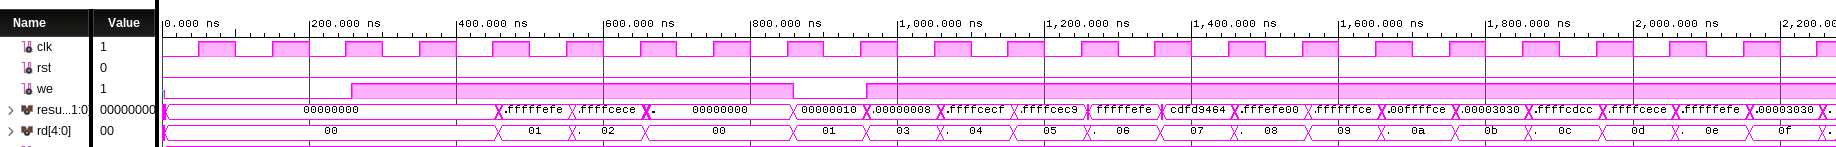
\includegraphics[width=\textwidth]{img/impl_10Mhz}
        \caption{Timing simulation at 10Mhz - Pass}
        %! suppress = FigureNotReferenced
        \label{fig:demo1}
	\end{figure}
    
	\begin{figure}[h!]
        \centering
        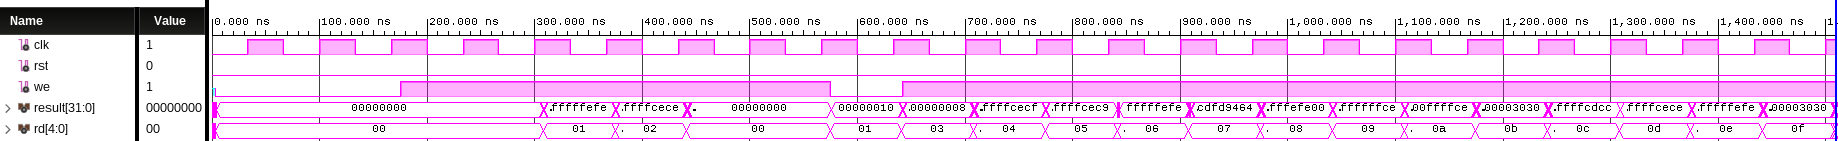
\includegraphics[width=\textwidth]{img/impl_15Mhz}
        \caption{Timing simulation at 15Mhz - Pass}
        %! suppress = FigureNotReferenced
        \label{fig:demo1}
	\end{figure}
    
	\begin{figure}[h!]
        \centering
        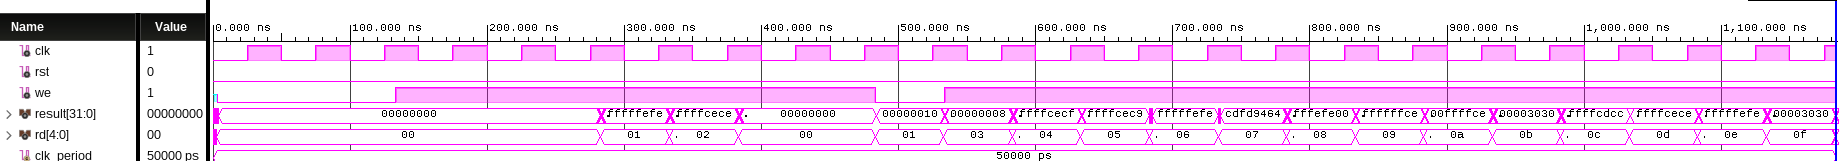
\includegraphics[width=\textwidth]{img/impl_20Mhz}
        \caption{Timing simulation at 20Mhz - Pass}
        %! suppress = FigureNotReferenced
        \label{fig:demo1}
	\end{figure}
    
	\begin{figure}[h!]
        \centering
        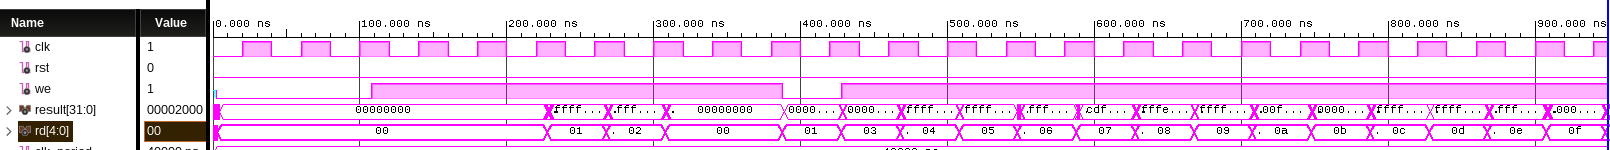
\includegraphics[width=\textwidth]{img/impl_25Mhz}
        \caption{Timing simulation at 25Mhz - Pass}
        %! suppress = FigureNotReferenced
        \label{fig:demo1}
	\end{figure}
    
	\begin{figure}[h!]
        \centering
        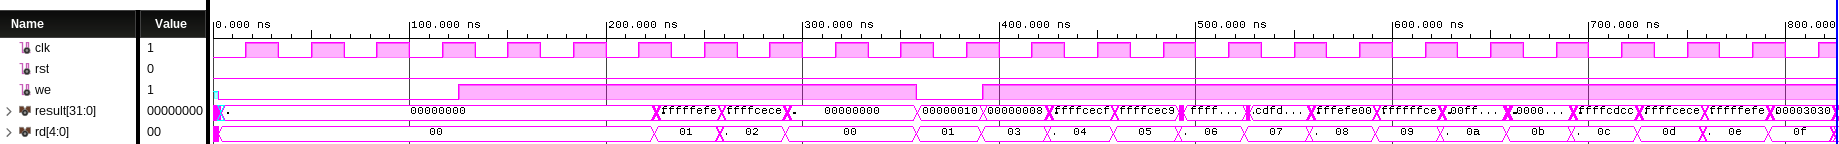
\includegraphics[width=\textwidth]{img/impl_30Mhz}
        \caption{Timing simulation at 30Mhz - Pass}
        %! suppress = FigureNotReferenced
        \label{fig:demo1}
	\end{figure}
    
	\begin{figure}[h!]
        \centering
        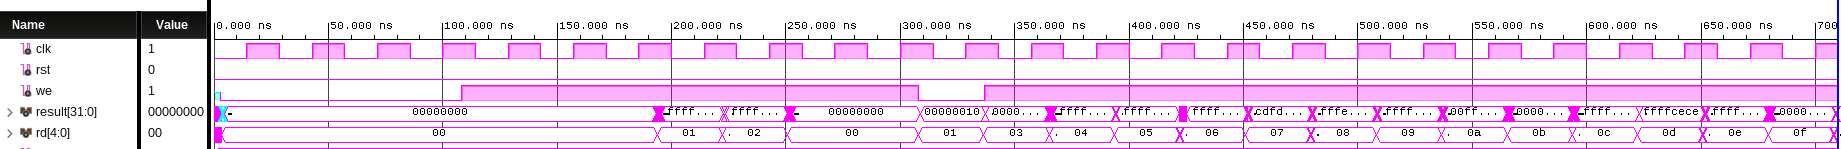
\includegraphics[width=\textwidth]{img/impl_35Mhz}
        \caption{Timing simulation at 35Mhz - Pass}
        %! suppress = FigureNotReferenced
        \label{fig:demo1}
	\end{figure}
    
	\begin{figure}[h!]
        \centering
        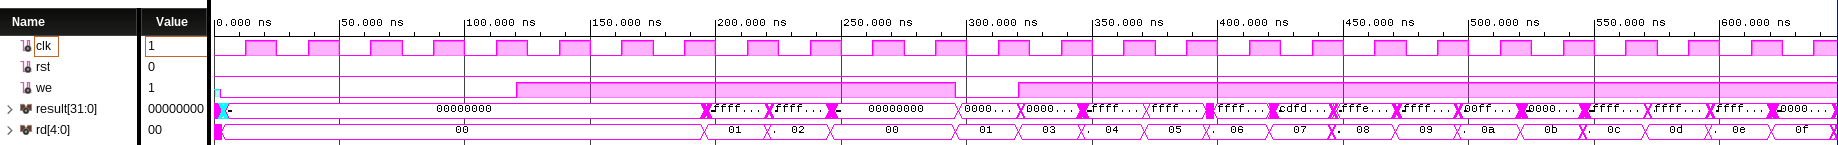
\includegraphics[width=\textwidth]{img/impl_40Mhz}
        \caption{Timing simulation at 40Mhz - Pass}
        %! suppress = FigureNotReferenced
        \label{fig:demo1}
	\end{figure}
    
	\begin{figure}[h!]
        \centering
        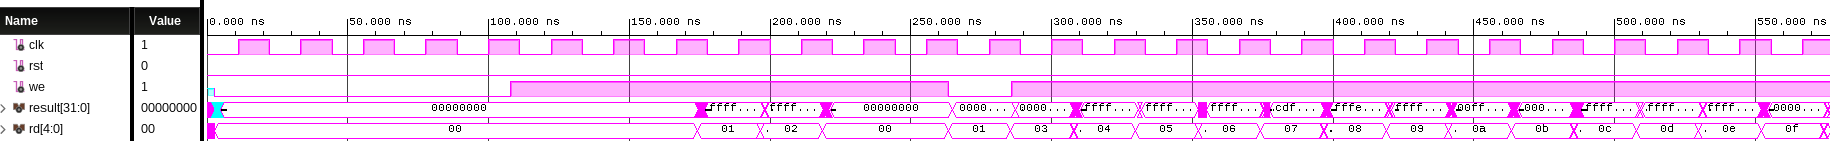
\includegraphics[width=\textwidth]{img/impl_45Mhz}
        \caption{Timing simulation at 45Mhz - Pass}
        %! suppress = FigureNotReferenced
        \label{fig:demo1}
	\end{figure}
    
	\begin{figure}[h!]
        \centering
        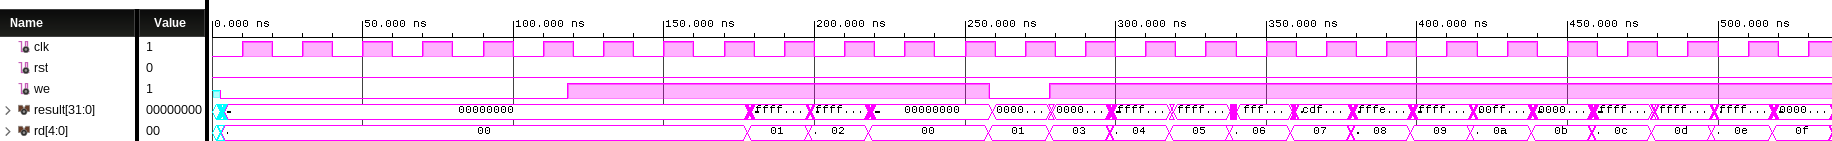
\includegraphics[width=\textwidth]{img/impl_50Mhz}
        \caption{Timing simulation at 50Mhz - Fail}
        %! suppress = FigureNotReferenced
        \label{fig:demo1}
	\end{figure}

\end{document}